\SubProblem
{هسته اصلی برنامه و رمزگشای مستوی}
{
\begin{figure}[H]
    \centering
    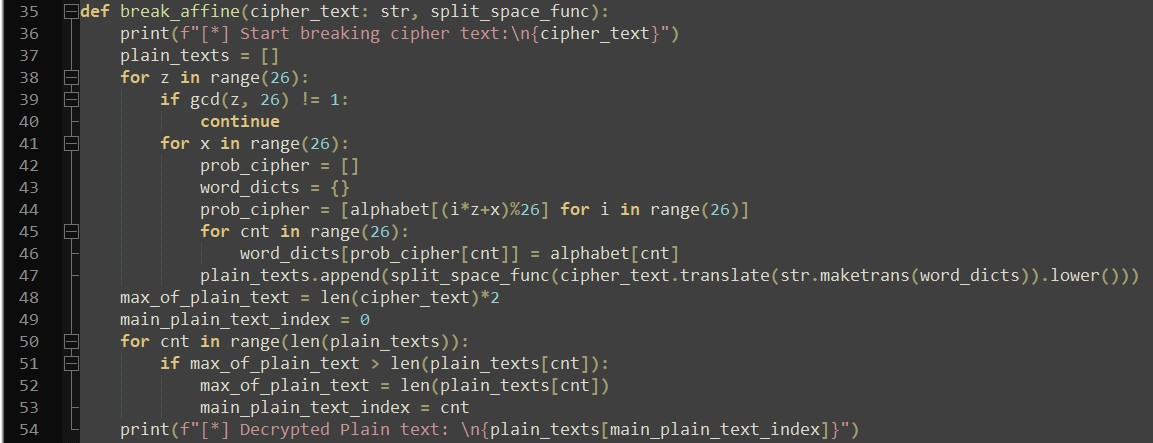
\includegraphics[width=15cm]{Images/F4.jpg}
    \label{fig:label}
    \caption{رمزگشای مستوی}
\end{figure}

در این قسمت طبق فرمولی که برای رمزگشایی مستوی ارائه دادیم عمل می‌شود.
هر بار که کلید جدیدی ساخته می‌شود با انجام فاصله گذاری‌های مختلف سعی می‌شود بهترین فاصله گذاری به ازای آن کلید پیدا شود. سپس میزان بهینه بودن آن متن پیدا شده محاسبه شده و نگه داشته می‌شود. هنگامی که متنی با بهینگی بهتر پیدا شد آن را به عنوان متن بهتر ذخیره می‌کنیم.
در نهایت بهترین متن خروجی داده می‌شود.
}
